\documentclass[a4paper]{article}
\usepackage{ucs}
\usepackage[utf8x]{inputenc}
\usepackage{changepage}
\usepackage{graphicx}
\usepackage{amsmath}
\usepackage{gensymb}
\usepackage{amssymb}
\usepackage{enumerate}
\usepackage{tabularx}
\usepackage{lipsum}
\usepackage{amsthm}
\usepackage{thmtools}
\usepackage{fancyvrb}


%% COLORED TABLES
\usepackage{colortbl}% http://ctan.org/pkg/colortbl
\usepackage{xcolor}% http://ctan.org/pkg/xcolor
\usepackage{booktabs}
\newcommand{\ra}[1]{\renewcommand{\arraystretch}{#1}}
\colorlet{tableheadcolor}{gray!25} % Table header colour = 25% gray
\newcommand{\headcol}{\rowcolor{tableheadcolor}} %
\colorlet{tablerowcolor}{gray!10} % Table row separator colour = 10% gray
\newcommand{\rowcol}{\rowcolor{tablerowcolor}} %
\usepackage{multirow}


\usepackage{fontspec} % loaded by polyglossia, but included here for transparency
\usepackage{polyglossia}




\makeatletter
\def\legendre@dash#1#2{\hb@xt@#1{%
  \kern-#2\p@
  \cleaders\hbox{\kern.5\p@
    \vrule\@height.2\p@\@depth.2\p@\@width\p@
    \kern.5\p@}\hfil
  \kern-#2\p@
  }}
\def\@legendre#1#2#3#4#5{\mathopen{}\left(
  \sbox\z@{$\genfrac{}{}{0pt}{#1}{#3#4}{#3#5}$}%
  \dimen@=\wd\z@
  \kern-\p@\vcenter{\box0}\kern-\dimen@\vcenter{\legendre@dash\dimen@{#2}}\kern-\p@
  \right)\mathclose{}}
\newcommand\legendre[2]{\mathchoice
  {\@legendre{0}{1}{}{#1}{#2}}
  {\@legendre{1}{.5}{\vphantom{1}}{#1}{#2}}
  {\@legendre{2}{0}{\vphantom{1}}{#1}{#2}}
  {\@legendre{3}{0}{\vphantom{1}}{#1}{#2}}
}
\def\dlegendre{\@legendre{0}{1}{}}
\def\tlegendre{\@legendre{1}{0.5}{\vphantom{1}}}
\makeatother



%\usepackage{xeCJK}
%\setCJKmainfont{SimSun}
%\setmainlanguage{russian}
%\setotherlanguage{english}

%\newfontfamily\cyrillicfont[Script=Cyrillic]{Times New Roman}
%\newfontfamily\cyrillicfontsf[Script=Cyrillic]{Arial}
%\newfontfamily\cyrillicfonttt[Script=Cyrillic]{Courier New}

\oddsidemargin -1.27cm
\evensidemargin -1.27cm
%\textwidth 6.27in
\textwidth 18.46cm
\topmargin -1.27cm
\headheight 0.0cm
\headsep 0.0cm
\textheight 27.16cm

\setlength\parindent{0pt}




% http://tex.stackexchange.com/questions/196961/thmtools-declaration-for-theorem-and-proof
\declaretheoremstyle[headfont=\normalfont\bfseries,notefont=\mdseries\bfseries,bodyfont = \normalfont,headpunct={:}]{normalhead}
\declaretheorem[name={Uzdevums}, style=normalhead,numberwithin=section]{problem}

\def\changemargin#1#2{\list{}{\rightmargin#2\leftmargin#1}\item[]}
\let\endchangemargin=\endlist


\newcommand{\subf}[2]{%
  {\small\begin{tabular}[t]{@{}c@{}}
  #1\\#2
  \end{tabular}}%
}



\newcounter{alphnum}
\newenvironment{alphlist}{\begin{list}{(\Alph{alphnum})}{\usecounter{alphnum}\setlength{\leftmargin}{2.5em}} \rm}{\end{list}}

\newenvironment{zhtext}{\fontfamily{MS PGothic}\selectfont}{\par}


\makeatletter
\let\saved@bibitem\@bibitem
\makeatother

\usepackage{bibentry}
\usepackage{hyperref}

\pagenumbering{gobble} 


\begin{document}




\arrayrulecolor[HTML]{DB5800}
\renewcommand{\arraystretch}{1.2}
\begin{table}[ht!]\centering
{\footnotesize
\begin{tabular*}{18.46cm}{@{}|p{2cm}p{6.35cm}|p{2cm}p{6.35cm}|@{}} \hline    
\headcol \multicolumn{4}{|c|}{\bf \normalsize Ģeometrijas faktu lapa (NMS)} \\ \hline 

\rowcol\multicolumn{4}{|p{18.01cm}|}{\textbf{1. Leņķu izteikšana.}  } \\ \hline 

& 
\cellcolor[HTML]{FFFFEE}
\textbf{Paralēlu taišņu leņķi:} Pie paralēlām taisnēm iekšējie šķērsleņķi un kāpšļu leņķi ir vienādi. 
Krustiskām taisnēm blakusleņķu summa ir $180^\circ$, bet krustleņķi ir vienādi. & 
\vspace{0pt} 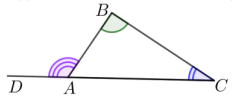
\includegraphics[width=1.9cm]{fig1-internal-external-angles.png} & 
\cellcolor[HTML]{FFFFEE} 
\textbf{Trijstūra ārējais leņķis} ir vienāds ar divu atlikušo iekšējo leņķu summu: 
$\sphericalangle BAD = \sphericalangle ABC + \sphericalangle BCA$. 
\\ \hline 
& 
\cellcolor[HTML]{FFFFEE}
\textbf{Iekšējo leņķu summa:} Trijstūra iekšējo leņķu summa ir $180^\circ$. Jebkura 
$n$-stūra iekšējo leņķu summa ir $(n-2) \cdot 180^\circ$. & 
& 
\cellcolor[HTML]{FFFFEE}
\textbf{Vienādsānu trijstūris:} Leņķi pie pamata ir vienādi tad un tikai tad, 
ja divas sānu malas ir vienādas. \\ \hline 

\rowcol\multicolumn{4}{|p{18.01cm}|}{\textbf{2. Laukums un metriskās sakarības.} } \\ \hline 

\multicolumn{2}{|p{8.787cm}|}{
\cellcolor[HTML]{FFFFEE}
\textbf{Trijstūra laukums}:\newline
$S_\Delta = \frac{1}{2}ah_a = pr = \frac{abc}{4R} = \frac{1}{2}ab \sin \gamma$ \newline 
{\bf Hērona formula}: $S_\Delta = \sqrt{p(p-a)(p-b)(p-c)}$, \newline
kur $a, b, c$ -- trijstūra malas, $\gamma$ -- leņķis starp $a$ un $b$, 
$h_a$ -- augstums, kas vilkts pret malu $a$, 
$p$ -- trijstūra pusperimetrs, 
$r$ -- ievilktās riņķa līnijas rādiuss, 
$R$ -- apvilktās riņķa līnijas rādiuss.
} &
\multicolumn{2}{p{8.787cm}|}{
\cellcolor[HTML]{FFFFEE}
\textbf{Regulārs trijstūris:} Ja regulāra trijstūra malas garums ir $a$, tad tā laukums $S_\Delta = \frac{a^2\sqrt{3}}{4}$, augstums $h = \frac{a\sqrt{3}}{2}$, ievilktās riņķa līnijas rādiuss $r = \frac{1}{3}h = \frac{a\sqrt{3}}{6}$, apvilktās riņķa līnijas rādiuss $R = \frac{2}{3}h = \frac{a\sqrt{3}}{3}$.
} \\ \hline

& 
\cellcolor[HTML]{FFFFEE}
\textbf{Laukumu attiecība (Ratio Lemma):} Trijstūrī $ABC$, ja punkts $D$ atrodas uz malas $BC$, tad dalot pamatu attiecībā $BD:CD$, arī laukumu attiecība ir $\frac{S(ABD)}{S(ACD)} = \frac{BD}{CD}$. Trijstūriem ar vienādu augstumu laukumi attiecas kā to pamatu garumi.
& 
& 
\cellcolor[HTML]{FFFFEE}
\textbf{Pitagora teorēma:} Taisnleņķa trijstūrim $a^2 + b^2 = c^2$. Trijstūra lielākais leņķis pret garāko malu $c$ ir šaurs, ja $a^2 + b^2 > c^2$, un plats, ja $a^2 + b^2 < c^2$. 
\\ \hline

\rowcol\multicolumn{4}{|p{18.01cm}|}{\textbf{3. Trijstūru vienādība un līdzība.} } \\ \hline 

& 
\cellcolor[HTML]{FFFFEE}
\textbf{Trijstūru vienādības pazīmes:} Divi trijstūri ir vienādi (sakrīt visi elementi), ja tiem sakrīt:
1) divas malas un leņķis starp tām (MML);
2) mala un divi pieguļošie leņķi (LML);
3) visas trīs malas (MMM).
& 
\vspace{0pt} 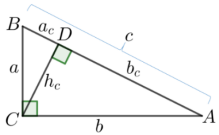
\includegraphics[width=1.9cm]{fig2-right-triangle_and_altitude.png} &
\cellcolor[HTML]{FFFFEE} 
No taisnleņķa trijstūra taisnā leņķa novilktais {\em augstums} $h_c$ sadala trijstūri divos taisnleņķa trijstūros, kas līdzīgi sākotnējam. 
\\ \hline

& 
\cellcolor[HTML]{FFFFEE}
\textbf{Trijstūru līdzības pazīmes:} Divi trijstūri ir līdzīgi (leņķi sakrīt, malas proporcionālas), ja:\newline
(1) divi leņķi ir vienādi (pazīme $\ell\ell$); \newline
(2) divas malas proporcionālas un leņķis starp tām vienāds (pazīme $m\ell m$); \newline
(3) trīs malas ir proporcionālas (pazīme $mmm$).
& 
& 
\cellcolor[HTML]{FFFFEE}
\textbf{Līdzīgu \boldmath{$\Delta$} īpašības:} Ja $\Delta_1 \sim \Delta_2$ un līdzības koeficients ir $k$ (malu attiecība ir $k$), tad to atbilstošo lineāro elementu (augstumu, perimetru, bisektrišu, mediānu) attiecība arī ir $k$. Laukumu attiecība ir $k^2$.
\\ \hline

\rowcol\multicolumn{4}{|p{18.01cm}|}{\textbf{4. Riņķa līnija.} } \\ \hline 

& 
\cellcolor[HTML]{FFFFEE}
\textbf{Centra un ievilktais leņķis:} Ievilktā leņķa lielums (virsotne atrodas uz riņķa līnijas) ir precīzi divas reizes mazāks par atbilstošā centra leņķa lielumu, kas balstās uz to pašu loku. 
& 
& 
\cellcolor[HTML]{FFFFEE}
\textbf{Taurenīša teorēma:} Visi ievilktie leņķi, kas balstās uz viena un tā paša loka, ir savā starpā vienādi. Regulējoša īpašība: ievilktais leņķis, kas balstās uz \textbf{diametru}, vienmēr ir $90^\circ$.
\\ \hline

& 
\cellcolor[HTML]{FFFFEE}
Četrstūrim \textbf{var apvilkt} riņķa līniju tad un tikai tad, ja tā pretējo 
leņķu summa ir $180^\circ$ ($\alpha + \gamma = \beta + \delta = 180^\circ$). 
& 
& 
\cellcolor[HTML]{FFFFEE}
Četrstūrī \textbf{var ievilkt} riņķa līniju tad un tikai tad, ja tā pretējo 
malu garumu summas ir vienādas ($a + c = b + d$).
\\ \hline

\rowcol\multicolumn{4}{|p{18.01cm}|}{\textbf{5. Ģeometriskie pārveidojumi.} } \\ \hline 

& 
\cellcolor[HTML]{FFFFEE}
\textbf{Pārnese un simetrija:} 
Paralēlā pārnese pārbīda visus plaknes punktus par noteiktu vektoru $\vec{v}$. 
Centrālā simetrija ir pagrieziens par $180^\circ$ ap simetrijas centru. 
Aksiālā simetrija pārveido punktu pret simetrijas taisni kā pret spoguli.
& 
& 
\cellcolor[HTML]{FFFFEE}
\textbf{Pagrieziens un homotētija:} 
Pagrieziens orientētā leņķī $\alpha$ ap centru $O$. 
Homotētija izmaina attālumus no dotā centra $O$ precīzi $k$ reizes. Tā vienmēr veido \textbf{līdzīgas} figūras (ja koeficients ir $k$, laukumi mainās $k^2$ reizes).
\\ \hline

\end{tabular*}
}
\end{table}

\end{document}
